\documentclass[sigconf]{acmart}

\acmConference{Master-Seminar}{Aktuelle Trends in der Systemsoftware}{SoSe 2026}

\settopmatter{
printacmref=false,
printccs=false,
printfolios=false
}
\renewcommand\footnotetextcopyrightpermission[1]{}
\usepackage{microtype}
\usepackage{booktabs}
\usepackage{array}
\usepackage{xcolor}
\usepackage{tikz}
\usepackage{listings}
\usetikzlibrary{arrows.meta, positioning, fit, calc}

\lstdefinestyle{commandstyle}{
basicstyle=\ttfamily\small,
breaklines=true,
columns=fullflexible,
frame=single
}

\urlstyle{tt}
\DeclareRobustCommand{\code}[1]{\path{#1}}

% Inline component labels matching the Temeraire component figure.
\newcommand{\compbox}[2]{%
\tikz[baseline=(X.base)]%
\node[
rounded corners=2pt,
inner xsep=3pt,
inner ysep=1.5pt,
draw=#1!70!black,
fill=#1!12,
line width=0.45pt
] (X) {\texttt{\footnotesize #2}};%
}

\newcommand{\HugeAllocatorLabel}{\compbox{blue}{HugeAllocator}}
\newcommand{\HugeCacheLabel}{\compbox{violet}{HugeCache}}
\newcommand{\HugeFillerLabel}{\compbox{green}{HugeFiller}}
\newcommand{\HugeRegionLabel}{\compbox{orange}{HugeRegion}}
\newcommand{\HugePageAwareAllocatorLabel}{\compbox{blue}{HugePageAwareAllocator}}

\definecolor{myblue}{HTML}{4C78A8}
\definecolor{mybluefill}{HTML}{EAF2FB}
\definecolor{mygreen}{HTML}{59A14F}
\definecolor{mygreenfill}{HTML}{EDF7EC}
\definecolor{myorange}{HTML}{F28E2B}
\definecolor{myorangefill}{HTML}{FDF1E3}
\definecolor{mygrayfill}{HTML}{F4F4F4}
\definecolor{myborder}{HTML}{666666}

\tikzset{
used/.style={
draw=myborder,
fill=mybluefill,
rounded corners=1.5pt,
minimum height=0.55cm,
minimum width=0.82cm
},
free/.style={
draw=myborder,
fill=mygrayfill,
rounded corners=1.5pt,
minimum height=0.55cm,
minimum width=0.82cm
},
component/.style={
draw=myblue,
fill=mybluefill,
rounded corners=3pt,
line width=0.8pt,
minimum height=0.78cm,
minimum width=2.2cm,
font=\scriptsize,
align=center,
inner sep=3pt
},
componentAlt/.style={
draw=mygreen,
fill=mygreenfill,
rounded corners=3pt,
line width=0.8pt,
minimum height=0.78cm,
minimum width=2.2cm,
font=\scriptsize,
align=center,
inner sep=3pt
},
cacheboxSmall/.style={
draw=myorange,
fill=myorangefill,
rounded corners=3pt,
line width=0.8pt,
minimum height=0.65cm,
minimum width=1.65cm,
font=\scriptsize,
align=center,
inner sep=2.5pt
},
labelbox/.style={
font=\scriptsize,
text=myborder
},
arrow/.style={
-{Latex[length=2.2mm,width=1.5mm]},
line width=0.8pt,
draw=myborder
}
}

\begin{document}
\raggedbottom

\title{Reproducing the Temeraire Redis Results on WSL2 and Bare-Metal Linux}

\author{Aldo Costa}
\email{aldo.costa@hhu.de}
\affiliation{%
\institution{Heinrich-Heine-Universit\"at}
\city{D\"usseldorf}
\state{Nordrhein-Westfalen}
\country{Deutschland}
}

\renewcommand{\shortauthors}{Costa}

\begin{abstract}
Temeraire is a hugepage-aware extension of TCMalloc that aims to improve
application performance by preserving hugepage coverage and reducing TLB
pressure. The original OSDI~2021 paper evaluates Temeraire through
application studies, a Google fleet experiment, and a production rollout.
This report deliberately narrows reproduction to the part that can be
approximated with public code: the Redis~6.0.9 case study.

The artifact evolved from a generic allocator benchmark into a Redis-focused
reproduction by pinning Redis, selecting a historical public TCMalloc revision,
building separate legacy and hugepage-aware shared libraries, and checking the
loaded allocator at runtime. Reaching a trustworthy measurement took two
environments and two series. Docker/WSL2 drifted by more than 200~kRPS while the
allocator was held constant, and the first bare-metal series recorded no CPU time
even though the paper normalizes its throughput for CPU.

The corrected series reproduces the paper's release-on result. Across four
balanced pairs the Temeraire delta is $+0.401\%$ in raw throughput and
$+0.474\%$ in requests per CPU second. All four pairs are positive, and both
95\% intervals exclude zero while containing the paper's $+0.44\%$.
Release-off centres on zero and stays unresolved
across two independent samples. Normalization proves to be worth under a tenth of
a percentage point here, because a single-threaded Redis under a saturating
benchmark holds one core throughout, and the release rate the paper omits matters
more than the metric: at 64~MiB/s every pair favors the legacy pageheap.
\end{abstract}

\begin{CCSXML} <ccs2012> <concept>
<concept_id>10011007.10010940.10010941.10010949.10010950</concept_id>
<concept_desc>Software and its engineering~Memory management</concept_desc>
<concept_significance>500</concept_significance> </concept> <concept>
<concept_id>10010520.10010575.10010755</concept_id>
<concept_desc>Computer systems organization~Reliability</concept_desc>
<concept_significance>300</concept_significance> </concept> </ccs2012>
\end{CCSXML}

\ccsdesc[500]{Software and its engineering~Memory management}
\ccsdesc[300]{Computer systems organization~Reliability}

\maketitle

\section{Introduction}

Memory allocation is often treated as a local implementation detail of C and
C++ programs. Temeraire starts from a different observation: allocator decisions
shape where objects land in memory, whether huge pages remain usable, and how
much address-translation work the processor must perform later. Hunter et al.
therefore connect allocator design to fleet efficiency as well as the direct
cost of \code{malloc} and \code{free} \cite{273711}.

A full reproduction of the Temeraire paper is outside the scope of this seminar
artifact. The paper's main evidence comes from Google's production environment,
including internal workloads, large-scale telemetry, and fleet-level rollout
data. Those conditions are not available externally. This report therefore
focuses on the Redis~6.0.9 case study: a public workload where the paper gives
enough benchmark detail to support a local reproduction attempt.

The question here is narrower than rebuilding Google's internal allocator
binary: can the Redis comparison be approximated with public code closely enough
to observe the same small-effect regime? Reaching that point required two
environments. Docker/WSL2 provided the development and diagnostic stage; a
dedicated Linux node provided the final native measurements.

\section{Background and Temeraire Mechanism}
\label{sec:background-temeraire}

Processors translate virtual addresses to physical addresses through page
tables. Because page-table walks are expensive, recent translations are cached
in translation lookaside buffers (TLBs). With ordinary 4~KiB pages, large
working sets can require many translations. A 2~MiB hugepage covers the same
address range as 512 ordinary pages, so one hugepage TLB entry can cover much
more memory than one ordinary-page entry.

The gain comes from needing fewer cached translations, not from loading 2~MiB of
data into cache at once. Whether that gain is realized depends on layout:
hugepage mappings require suitably aligned and contiguous regions. Linux
Transparent Huge Pages (THP) can create such mappings, but its success depends
partly on how the user-space allocator arranges live objects.

\begin{figure}[t]
\centering
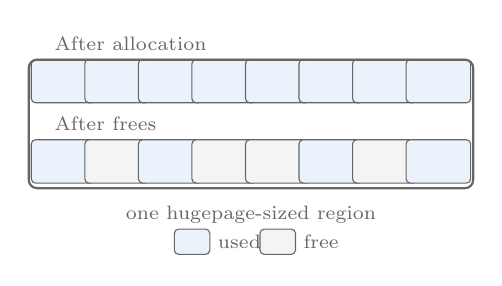
\begin{tikzpicture}[x=0.68cm,y=0.68cm]
\node[labelbox, anchor=west] at (-0.35,2.45) {After allocation};
\node[labelbox, anchor=west] at (-0.35,0.95) {After frees};

\foreach \i in {0,...,7} { \node[used] at (\i,1.75) {}; }

\node[used] at (0,0.25) {};
\node[free] at (1,0.25) {};
\node[used] at (2,0.25) {};
\node[free] at (3,0.25) {};
\node[free] at (4,0.25) {};
\node[used] at (5,0.25) {};
\node[free] at (6,0.25) {};
\node[used] at (7,0.25) {};

\draw[draw=myborder, line width=0.8pt, rounded corners=3pt]
  (-0.65,-0.25) rectangle (7.65,2.15);
\node[labelbox] at (3.5,-0.75) {one hugepage-sized region};

\node[used, minimum width=0.45cm, minimum height=0.32cm] at (2.4,-1.25) {};
\node[labelbox, anchor=west] at (2.7,-1.25) {used};
\node[free, minimum width=0.45cm, minimum height=0.32cm] at (4.0,-1.25) {};
\node[labelbox, anchor=west] at (4.3,-1.25) {free};

\end{tikzpicture}
\caption{Fragmentation inside a hugepage-sized region. Free memory exists,
but live objects prevent the whole region from being released intact. Redrawn
after Figure~1 in Hunter et al.~\cite{273711}.}
\Description{A hugepage-sized memory region before and after free operations,
showing used blocks separated by fragmented free blocks.}
\label{fig:fragmentation}
\end{figure}

Figure~\ref{fig:fragmentation} shows the central trade-off. Returning small
free pieces to the OS can reduce resident memory, but it may split hugepage
mappings. Keeping the hugepage intact preserves TLB coverage, but leaves some
physical memory idle. Temeraire exists to make this trade-off explicit inside
the allocator backend.

TCMalloc is organized as a hierarchy of caches. Many small allocations are
served by upper per-CPU, transfer, or central-cache layers. Larger
page-granularity requests eventually reach the pageheap, which obtains memory
from the OS and releases unused spans. Temeraire modifies this backend pageheap
layer rather than replacing the whole allocator.

\begin{figure}[t]
\centering
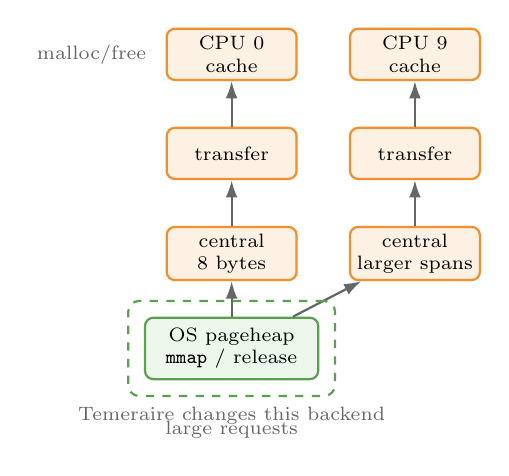
\begin{tikzpicture}[node distance=0.55cm and 0.65cm]
\node[componentAlt] (os) {OS pageheap\\\texttt{mmap} / release};

\node[cacheboxSmall, above=0.45cm and 0.75cm of os] (central8) {central\\8 bytes};
\node[cacheboxSmall, right=0.65cm of central8] (centralbig) {central\\larger spans};

\node[cacheboxSmall, above=0.58cm of central8] (transfer8) {transfer};
\node[cacheboxSmall, above=0.58cm of centralbig] (transferbig) {transfer};

\node[cacheboxSmall, above=0.58cm of transfer8] (cpu0) {CPU 0\\cache};
\node[cacheboxSmall, above=0.58cm of transferbig] (cpu9) {CPU 9\\cache};

\draw[arrow] (os) -- (central8);
\draw[arrow] (os) -- (centralbig);
\draw[arrow] (central8) -- (transfer8);
\draw[arrow] (centralbig) -- (transferbig);
\draw[arrow] (transfer8) -- (cpu0);
\draw[arrow] (transferbig) -- (cpu9);

\node[labelbox, left=0.12cm of cpu0] {malloc/free};
\node[labelbox, below=0.40cm of os] {large requests};

\node[
  draw=mygreen,
  dashed,
  rounded corners=4pt,
  line width=0.8pt,
  fit=(os),
  inner sep=0.20cm,
  label={[labelbox]below:Temeraire changes this backend}
] {};

\end{tikzpicture}
\caption{Simplified TCMalloc hierarchy. Temeraire changes the backend
pageheap layer while leaving the upper cache structure intact. Redrawn after
Figure~3 in Hunter et al.~\cite{273711}.}
\Description{A simplified hierarchy from CPU caches through transfer and
central caches down to the OS pageheap.}
\label{fig:tcmalloc}
\end{figure}

This localization sets the shape of the reproduction. The experiment compares two
backend configurations of one allocator, the legacy pageheap and the
hugepage-aware path, rather than two separate allocators.

\begin{figure}[t]
\centering
\resizebox{\columnwidth}{!}{%
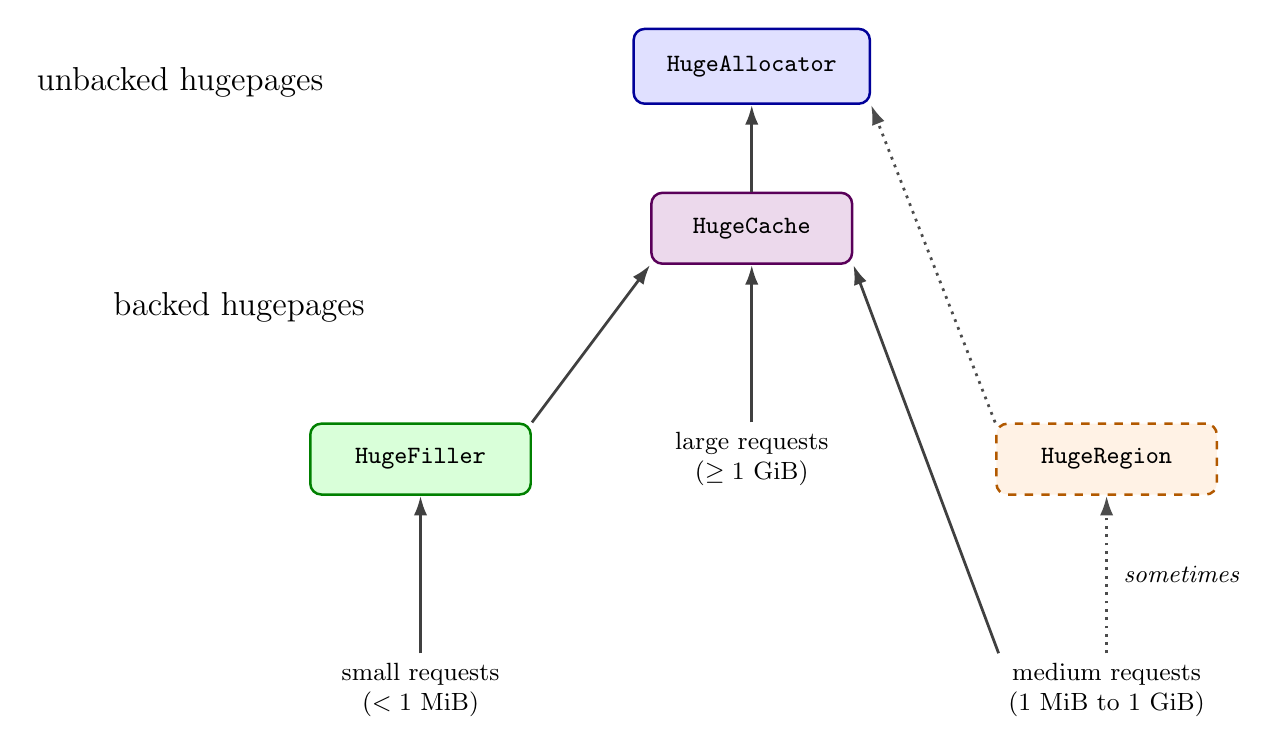
\begin{tikzpicture}[
>=Latex,
font=\scriptsize,
node distance=0.8cm and 1.2cm,
every node/.style={align=center}
]

\tikzset{
  allocatorbox/.style={
    draw=blue!60!black,
    fill=blue!12,
    rounded corners=4pt,
    line width=0.9pt,
    minimum width=3.0cm,
    minimum height=0.95cm,
    font=\small\ttfamily
  },
  cachebox/.style={
    draw=violet!70!black,
    fill=violet!15,
    rounded corners=4pt,
    line width=0.9pt,
    minimum width=2.55cm,
    minimum height=0.9cm,
    font=\small\ttfamily
  },
  fillerbox/.style={
    draw=green!50!black,
    fill=green!15,
    rounded corners=4pt,
    line width=0.9pt,
    minimum width=2.8cm,
    minimum height=0.9cm,
    font=\small\ttfamily
  },
  regionbox/.style={
    draw=orange!70!black,
    fill=orange!10,
    rounded corners=4pt,
    dashed,
    line width=0.9pt,
    minimum width=2.8cm,
    minimum height=0.9cm,
    font=\small\ttfamily
  },
  solidflow/.style={
    -{Latex[length=2.5mm,width=1.7mm]},
    line width=1.0pt,
    draw=black!75
  },
  dottedflow/.style={
    -{Latex[length=2.5mm,width=1.7mm]},
    dotted,
    line width=1.0pt,
    draw=black!70
  },
  textlabel/.style={
    font=\small,
    text=black
  },
  biglabel/.style={
    font=\large,
    text=black
  }
}

\node[allocatorbox] (allocator) {HugeAllocator};
\node[cachebox, below=1.1cm of allocator] (cache) {HugeCache};

\node[fillerbox, below left=2.0cm and 1.5cm of cache] (filler) {HugeFiller};
\node[regionbox, below right=2.0cm and 1.8cm of cache] (region) {HugeRegion};

\node[biglabel, left=3.8cm of allocator, yshift=-0.2cm] (unbacked) {unbacked hugepages};
\node[biglabel, left=3.5cm of cache, yshift=-1.0cm] (backed) {backed hugepages};

\draw[solidflow] (cache) -- (allocator);
\draw[solidflow] (filler.north east) -- (cache.south west);
\draw[dottedflow] (region.north west) -- (allocator.south east);

\node[textlabel, below=2.0cm of filler] (smallreq)
  {small requests\\($< 1$ MiB)};
\node[textlabel, below=2.0cm of cache] (largereq)
  {large requests\\($\geq 1$ GiB)};
\node[textlabel, below=2.0cm of region] (medreq)
  {medium requests\\($1$ MiB to $1$ GiB)};

\draw[solidflow] (smallreq.north) -- (filler.south);
\draw[solidflow] (largereq.north) -- (cache.south);
\draw[solidflow] (medreq.north west) -- (cache.south east);
\draw[dottedflow] (medreq.north) --
  node[right, textlabel, xshift=0.08cm] {\emph{sometimes}} (region.south);

\end{tikzpicture}%
}
\caption{Temeraire's component structure. Small requests are routed to
\code{HugeFiller}, large requests to \code{HugeCache}, and medium requests
usually to \code{HugeCache} but occasionally to \code{HugeRegion}. Adapted
after Figure~6 in Hunter et al.~\cite{273711}.}
\Description{A diagram of Temeraire components connecting HugeAllocator,
HugeCache, HugeFiller, and HugeRegion with request flows by allocation size.}
\label{fig:temeraire-components}
\end{figure}

Figure~\ref{fig:temeraire-components} summarizes the backend components relevant
for the artifact. \HugeAllocatorLabel{} manages hugepage-aligned virtual
address ranges. \HugeCacheLabel{} keeps completely empty backed hugepages for
reuse. \HugeFillerLabel{} handles small allocations and is the key component for
Redis. \HugeRegionLabel{} handles medium-sized allocations that would otherwise
create large slack regions.

The key Redis-relevant policy is in \HugeFillerLabel{}. For a request of size
$K$, it prefers a hugepage whose longest free run is just large enough for the
request. When several candidates are equivalent, it prefers the fuller one. This
avoids consuming long free runs unnecessarily and avoids disturbing nearly empty
hugepages that might otherwise drain and be released.

The Redis list workload in the paper performs small list-node and string-value
allocations. These do not reach \HugeFillerLabel{} individually. As
Figure~\ref{fig:tcmalloc} shows, the per-CPU and central caches serve them; only
when those caches need fresh backing spans does a page-level request arrive at
the pageheap. \HugeFillerLabel{} places those spans, and the legacy pageheap
places them without a hugepage-aware objective.
Section~\ref{sec:methodology} turns that difference into the measured
hypothesis.

Periodic memory release complicates the picture. When release is enabled,
TCMalloc can return memory to the OS using mechanisms such as
\code{MADV_DONTNEED}. Release interacts with hugepage coverage and adds
variance, so release-off carries the cleaner placement signal of the two
conditions.

\section{Reproduction Target and Artifact Evolution}
\label{sec:target-artifact}

The original paper reports application studies, a fleet experiment, and a
production rollout. Only the Redis case study is realistic for a public seminar
reproduction. The paper gives Redis~6.0.9, a legacy TCMalloc pageheap baseline,
2000 \code{redis-benchmark} trials, 1,000,000 requests per trial, and a workload
combining a five-element push with a five-element read \cite{273711}. It also
states the CPU family and LLVM commit used for compilation. The exact Linux
distribution, kernel version, and THP policy for the Redis run are left
unstated, so this report documents them locally instead of matching them.

The repository did not initially match this target. It was a useful allocator
benchmark scaffold, but its defaults used Redis~7.2.5, compared glibc against
open-source gperftools TCMalloc, and did not expose a clean legacy-pageheap
versus Temeraire comparison. The first reproduction step was to narrow and
correct the claim: the artifact would reproduce the Redis case-study methodology
only, not the paper's full evaluation.

The paper's internal allocator build is unavailable, so the artifact uses a
historical public \code{google/tcmalloc} commit, \code{8e534f507074}, which
still exposes the \code{want_no_hpaa} mechanism needed to disable the
hugepage-aware path. This makes a public legacy-versus-Temeraire split possible,
but it should not be read as byte-identical to Google's internal artifact.

The public repository provides no ready-made shared libraries for Redis
preloading. The setup script therefore adds a small wrapper target inside the
cloned TCMalloc tree and builds two loadable variants. The Temeraire build
links against \code{//tcmalloc}; the legacy build also links against
\code{//tcmalloc:want_no_hpaa}. The benchmark harness selects the desired
library through \code{LD_PRELOAD}.

Bazel was helpful because it let the artifact use TCMalloc's native build graph
instead of reconstructing allocator dependencies, compiler flags, and link
semantics in a separate build system. It also kept the comparison narrow: both
shared libraries are produced from the same wrapper source, and the intended
difference is the allocator target plus the extra \code{//tcmalloc:want_no_hpaa}
dependency in the legacy build. The cost was integration friction. Bazelisk had
to be installed and pinned, the exact LLVM compiler path had to be passed
through Bazel's action and repository environments, an external wrapper
workspace did not inherit the right dependencies, and target visibility forced
the wrapper into \code{tcmalloc/testing}.

Runtime verification is necessary. Redis reports
\texttt{mem\_allocator: libc} from its own build metadata even when
\code{LD_PRELOAD} has replaced the process allocator, so the artifact checks
\code{/proc/$pid/maps} to confirm that the intended shared library is mapped
into the Redis process.

The final artifact reflects several failed or revised approaches. A modern
\code{google/tcmalloc} checkout was not a convenient starting point for this
wrapper strategy, and an external Bazel wrapper workspace did not naturally
inherit all TCMalloc dependencies such as Abseil. The successful path was to add
the wrapper inside the cloned TCMalloc source tree. Visibility was another
obstacle: the \code{want_no_hpaa} target could not be linked from an arbitrary
external package, so the wrapper had to be placed where TCMalloc's own
visibility rules permitted the dependency.

A later validation run uncovered a symbol mismatch. The wrapper initially
referenced background-release methods that were not present in the pinned
historical TCMalloc revision. The shared objects built, but failed to load before
Redis started. The fix was to resolve those methods dynamically when available,
allowing the wrapper to load against the historical revision while preserving
the intended behavior for newer revisions.

Compiler matching also proved more expensive than it first looked. The paper
mentions LLVM commit \code{cd442157cf} and \code{-O3}. Matching that statement
required a local LLVM/clang toolchain, then using it for Redis, gperftools, and
the Bazel-based TCMalloc wrapper build. Later metadata confirmed use of a local
LLVM~13.0.0 build from the longer \code{cd442157cf} commit. One older manifest
still marked the exact LLVM path as disabled, so the compiler metadata is treated
as authoritative.

The most important methodological difficulty was THP. Initial long runs under
WSL2/Docker with THP in \code{madvise} mode recorded \texttt{AnonHugePages: 0 kB}
for Redis. These runs looked like controlled allocator comparisons while leaving
the hugepage mechanism itself unevidenced. The harness was then extended to
record THP settings and periodic \code{smaps_rollup} snapshots, and the final
paper-closer runs set THP to \code{always} before benchmarking. Even after that
correction, later release-on runs showed large changes in absolute host
throughput. That drift is what moved the same experiment to bare-metal Linux
instead of leaving the WSL2 measurements as the final result.

\section{Methodology}
\label{sec:methodology}

\subsection{Common benchmark path}

The repository retains a short direct Redis path for smoke tests and allocator
preload checks. Measurements reported here use the paper-closer path. It fixes
Redis to version~6.0.9 and uses 2000 trials, 50 clients, and pipeline depth~16.
Each trial flushes the database and then runs two separate
\code{redis-benchmark} invocations of 1,000,000 requests each:

\begin{itemize}
\item \texttt{LPUSH benchmark:list v1 v2 v3 v4 v5};
\item \texttt{LRANGE benchmark:list 0 4}.
\end{itemize}

This structure is one reading of an underspecified sentence, and its consequences
should be stated plainly. The paper specifies 2000 trials, each trial making one
million requests ``to push 5 elements and read those 5 elements''
\cite{273711}. Read literally, one request covers both the push and the read, so
a trial performs one million of each. The local trial instead issues one million
pushes and then one million reads, which doubles the command count to two
million. It also separates the phases: because all pushes precede all reads,
\texttt{LRANGE 0 4} returns the same final five elements on every read while the
list holds five million, rather than returning each group just after that group
was pushed. An interleaved implementation would keep the live set small and touch
freshly written memory, which is a different access pattern and a different
live-heap shape for the allocator under test. This report does not claim its
choice is the paper's; it records the choice so that the comparison can be judged
and repeated.

The runner stores the raw output of every operation as well as summary files,
Redis logs, memory snapshots, allocator order, software revisions, and system
metadata. Allocator order alternates between pairs. This does not remove drift
between two consecutive blocks, but it avoids assigning the same allocator to
the later position every time.

The primary metric is throughput in requests per second from
\code{redis-benchmark}. LPUSH and LRANGE are collapsed into a combined
push-plus-read rate using the harmonic mean
\[
  \frac{2}{1/r_{\mathrm{LPUSH}} + 1/r_{\mathrm{LRANGE}}}.
\]
This treats the two throughputs as rates for sequential operations and reduces
each block to one number, as the paper's single Redis delta per release mode
does. The harmonic-mean aggregation itself is not specified in the
paper. It is a local reconstruction choice because our public
\code{redis-benchmark} harness records LPUSH and LRANGE as separate operation
means, while the paper reports one Redis throughput delta for the combined
push-five/read-five workload.

This metric is not the paper's metric, and the difference bounds every comparison
in Section~\ref{sec:results}. The caption of Table~1 in Hunter et al. states that
throughput there is ``normalized for CPU'', and the surrounding text gives the
unit as requests per second per core \cite{273711}. The local figure is
unnormalized: it is the request rate \code{redis-benchmark} reports, divided by
nothing. A ratio of unnormalized rates cannot separate a genuine throughput gain
from the same throughput bought with more CPU, which is exactly the distinction
the paper's normalization preserves and the distinction its fleet-efficiency
argument rests on. The local aggregation across two operations compounds this,
since the paper reports no per-operation rates to compare against.

The consequence is stated once here and assumed afterwards. Where this report
places a local value near a published one, that is numerical proximity between
two differently constructed quantities. It is not agreement between two instances
of one measurement, and no local number in this report can confirm or contradict
the paper's normalized figures.

The hypothesis is modest, and follows from
Section~\ref{sec:background-temeraire}. If the placement heuristic in
\HugeFillerLabel{} improves hugepage coverage for the spans backing Redis's
small allocations, Redis should show a small positive throughput delta against
the legacy pageheap. The effect should be clearest with periodic release
disabled, since release-on adds interaction with background memory return and
can mask the placement signal.

\subsection{Docker/WSL2 development stage}

The first complete setup used a Debian~12 container on Docker Desktop and its
shared WSL2 kernel. It was where the pinned builds, preload checks, benchmark
parameters, THP instrumentation, and balanced ordering were developed. Once THP
was set to \code{always}, Redis reported non-zero hugepage use. The container
stayed a good development environment and made a poor measuring instrument, for
reasons Section~
ef{sec:earlier-series} gives.

Two faults found in that stage shaped everything after it. The runner started
TCMalloc's background-actions thread without setting a release rate, which the
pinned revision defaults to zero, so nothing labelled release-on had performed
periodic release. Fixing that exposed a second fault: the wrapper's dynamic
symbol lookups had been failing silently, and \code{LD\_PRELOAD} had leaked
from the Redis server to \code{redis-cli} and \code{redis-benchmark}, mixing
client and server allocators into the same comparison. The wrapper now calls the
linked TCMalloc API directly, the preload is scoped to the server, and every
release-on run must log its requested rate before the benchmark proceeds.

\subsection{Bare-metal Linux stage}

The WSL2 drift motivated a second workflow rather than a change to the existing
container scripts. The native scripts preserve the same pinned source revisions,
allocator wrappers, Redis workload, result layout, and balanced pair structure.
They run directly on the dedicated node described in
Table~\ref{tab:bare-metal-setup}.

\begin{table}[ht]
\caption{Recorded bare-metal environment on node85.}
\label{tab:bare-metal-setup}
\footnotesize
\begin{tabular}{@{}lp{0.57\columnwidth}@{}}
\toprule
Field & Recorded value \\
\midrule
OS & Debian GNU/Linux 13 (trixie) \\
Kernel & \code{6.12.95+deb13-amd64} \\
Processor & Intel Xeon Gold 5318N \\
Topology & 24 cores, 48 threads, one NUMA node \\
Memory & 188~GiB \\
Virtualization & none detected \\
THP & \code{always}; defrag \code{madvise} \\
\bottomrule
\end{tabular}
\end{table}

The move exposed a different set of practical problems. The shared home
directory was too slow for Bazel's many small files, so the build and runs were
moved to \code{/var/tmp}. The compute node could not fetch the pinned sources,
which meant staging source and dependency archives for an offline build. The old
LLVM revision also needed \texttt{-include cstdint} to build with Debian~13's
host compiler. Finally, the German locale produced decimal commas in CSV files;
the native runner now sets \code{LC_ALL=C}.

Three two-trial smoke runs and two ten-trial pilots came first. Four full
balanced pairs then ran at 16~MiB/s, each pair covering legacy and Temeraire
with release disabled and enabled. A second series kept release enabled and
added four order-alternated pairs at 64~MiB/s and four at 256~MiB/s. All full
allocator blocks contain 2000 trials, and each release-on Redis log confirms the
requested rate. The archive holds 64,000 trial rows for the main four pairs and
another 64,000 for the two added rates. A standard-library audit script
re-derives every block mean from the raw trial files, checks trial identifiers,
request counts, file counts, memory samples, THP state, release-rate
confirmations, clean shutdowns, allocator order, and system metadata, and fails
on any mismatch. Both halves of the archive pass.

\section{Results}
\label{sec:results}

\subsection{Why these are the second series of measurements}
\label{sec:why-rerun}

The first bare-metal series was complete and audited, and it was measuring the
wrong thing in ways that only became visible afterwards. Three problems surfaced,
in an order worth recording, because the last two were faults in the harness that
produced those very numbers.

The first came from reading the paper again with the harness open alongside it.
The caption of Table~1 in Hunter et al.\ says that its throughput is
``normalized for CPU'', and the surrounding text gives the unit as requests per
second per core \cite{273711}. The local figure was an unnormalized request
rate. A ratio of unnormalized rates cannot distinguish Temeraire serving more
requests from Temeraire serving the same requests at higher CPU cost, and the
artifact recorded no CPU time at all, so the distinction could not be recovered
from the archived runs. The same reading showed that the paper's trial, one
million requests ``to push 5 elements and read those 5 elements'', supports a
second implementation in which one request performs both operations, and that
the paper's Redis servers used Skylake Xeons while node85 carries an Ice Lake
part. Two of those three gaps could be closed by changing the harness. The
processor could not.

The second problem appeared eighteen hours into the first corrected attempt. A
block died at trial 1875 of 2000 with \texttt{Connection reset by peer}, and the
Redis log for that block showed a clean shutdown, which made the failure look
like a transient fault on a shared node. It was not. The run had been started
with a plain background \code{\&} from an interactive shell, so it stayed inside
the SSH session, and the session had ended. Redis ignores \code{SIGHUP} at
startup and \code{redis-benchmark} does not, so the hangup killed the client,
left the server running, and the script's exit trap then shut that server down
politely. The clean shutdown was the consequence of the failure rather than
evidence against it.

The third problem destroyed a whole day of compute and was entirely self
inflicted. \code{redis-benchmark} builds its CSV test name from the command
line, so a run driven by an \code{EVAL} script carries the whole Lua source in
that field, commas included. The harness read the rate by splitting the line on
commas and taking the second field, which for such a run is the fragment
\code{KEYS[1]}. Every trial of the first sixteen-hour block recorded that string,
and the block mean came out as zero. Plain \code{LPUSH} and \code{LRANGE} names
contain no commas, which is why the fault stayed hidden until the second workload
ran for the first time.

That last one was recoverable, because the runner writes each benchmark
invocation's output to its own file before deriving anything from it. Those files
held the correct rates the whole time, and a separate utility re-derives
\code{trials.csv} and \code{summary.csv} from them, so the sixteen hours were
repaired rather than repeated. The episode still points at a real weakness in the
audit: it compares the summary against the aggregated trial table, and both
descend from the same extraction, so it caught this only because \code{KEYS[1]}
is not a number. A plausible but wrong value would have passed.

Four changes came out of these problems. Each block now records the CPU time of
the Redis server from \texttt{redis-cli info cpu}, which is that block's total
because Redis restarts for every block. The workload is selectable, so both
readings of the paper's trial sentence can be measured instead of one being
chosen and defended. A failed benchmark invocation is retried, and every attempt
reaches the audit as a warning so a retried block cannot pass as a clean one.
Runs start in their own session through \code{setsid}, which removes the hangup
described above.

\subsection{Reported result}
\label{sec:reported-result}

The corrected series ran for 90.7 hours on node85 and produced eight balanced
pairs: four using the sequential workload of Section~\ref{sec:methodology}, and
four using the combined \code{EVAL} reading. Every block holds 2000 trials, every
release-on log confirms the 16~MiB/s rate, no block needed a retry, and the two
launcher status files record a zero exit code. Of the 32 blocks, 28 re-derive
byte-identical summaries from their raw per-trial files; the four that differ are
the block set damaged by the extraction fault, repaired as described above.

\begin{table}[ht]
\caption{Reported result. Correction run on node85, sequential workload. Deltas
in raw throughput and in requests per CPU second, the unit the paper reports.
Intervals are four-pair Student-t intervals on the log-transformed pair ratios
and accompany the mean.}
\label{tab:correction-sequential}
\footnotesize
\begin{tabular}{@{}lrrr@{}}
\toprule
Pair & Order & Release off & Release on \\
\midrule
5 & L first & $-0.476\%$ & $+0.242\%$ \\
6 & T first & $+0.156\%$ & $+0.555\%$ \\
7 & L first & $-0.083\%$ & $+0.380\%$ \\
8 & T first & $+0.490\%$ & $+0.426\%$ \\
\midrule
Mean            & & $+0.022\%$ & $+0.401\%$ \\
Median          & & $+0.037\%$ & $+0.403\%$ \\
95\% interval   & & $[-0.62,+0.67]$ & $[+0.20,+0.61]$ \\
\midrule
Mean per CPU second   & & $+0.091\%$ & $+0.474\%$ \\
95\% interval         & & $[-0.74,+0.93]$ & $[+0.30,+0.65]$ \\
\midrule
Paper           & & $+0.75\%$ & $+0.44\%$ \\
\bottomrule
\end{tabular}
\end{table}

Release-on at 16~MiB/s reproduces the paper. All four pairs favor Temeraire and
the mean is $+0.401\%$, with an interval that excludes zero. Normalizing for CPU
moves the mean to $+0.474\%$, and that interval excludes zero as well. The
paper's $+0.44\%$ falls inside both. This is the only condition in the study that
separates from the baseline in Temeraire's favor, and it does so in the paper's
own unit and within its reported value. Absolute throughput held between 980 and
995~kRPS across all sixteen blocks, a spread of $1.6\%$.

Release-off does not resolve. The mean is $+0.022\%$ and the median $+0.037\%$,
with an interval that covers zero and, once normalized, covers the paper's
$+0.75\%$ as well. Figure~\ref{fig:distributions} shows why four pairs are not
enough here: the per-trial distributions inside each block span roughly $4\%$,
an order of magnitude wider than the pairwise deltas that separate them, so the
allocator difference is a small shift between two heavily overlapping
populations.

\begin{figure}[t]
\centering
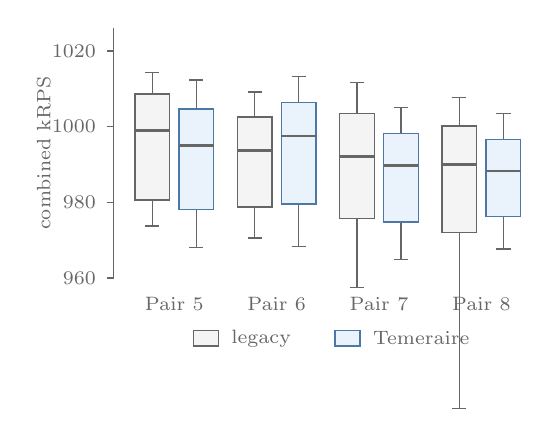
\begin{tikzpicture}[x=1cm, y=0.048cm]
\tikzset{
  whisker/.style={draw=myborder, line width=0.5pt},
  boxlegacy/.style={draw=myborder, fill=mygrayfill, line width=0.5pt},
  boxtemeraire/.style={draw=myblue, fill=mybluefill, line width=0.5pt},
  medianline/.style={draw=myborder, line width=1.0pt}
}

\draw[draw=myborder, line width=0.5pt] (0.38,0) -- (0.38,66);
\foreach \value/\offset in {960/0, 980/20, 1000/40, 1020/60} {
  \draw[draw=myborder, line width=0.5pt] (0.30,\offset) -- (0.38,\offset);
  \node[labelbox, anchor=east] at (0.28,\offset) {\value};
}
\node[labelbox, rotate=90, anchor=south] at (-0.30,33) {combined kRPS};

% pair 5, legacy
\draw[whisker] (0.870,13.75) -- (0.870,20.58);
\draw[whisker] (0.870,48.61) -- (0.870,54.27);
\draw[whisker] (0.780,13.75) -- (0.960,13.75);
\draw[whisker] (0.780,54.27) -- (0.960,54.27);
\draw[boxlegacy] (0.650,20.58) rectangle (1.090,48.61);
\draw[medianline] (0.650,39.02) -- (1.090,39.02);
% pair 5, temeraire
\draw[whisker] (1.430,8.10) -- (1.430,18.14);
\draw[whisker] (1.430,44.70) -- (1.430,52.30);
\draw[whisker] (1.340,8.10) -- (1.520,8.10);
\draw[whisker] (1.340,52.30) -- (1.520,52.30);
\draw[boxtemeraire] (1.210,18.14) rectangle (1.650,44.70);
\draw[medianline] (1.210,35.06) -- (1.650,35.06);
% pair 6, legacy
\draw[whisker] (2.170,10.57) -- (2.170,18.74);
\draw[whisker] (2.170,42.60) -- (2.170,49.19);
\draw[whisker] (2.080,10.57) -- (2.260,10.57);
\draw[whisker] (2.080,49.19) -- (2.260,49.19);
\draw[boxlegacy] (1.950,18.74) rectangle (2.390,42.60);
\draw[medianline] (1.950,33.69) -- (2.390,33.69);
% pair 6, temeraire
\draw[whisker] (2.730,8.24) -- (2.730,19.56);
\draw[whisker] (2.730,46.34) -- (2.730,53.24);
\draw[whisker] (2.640,8.24) -- (2.820,8.24);
\draw[whisker] (2.640,53.24) -- (2.820,53.24);
\draw[boxtemeraire] (2.510,19.56) rectangle (2.950,46.34);
\draw[medianline] (2.510,37.55) -- (2.950,37.55);
% pair 7, legacy
\draw[whisker] (3.470,-2.61) -- (3.470,15.75);
\draw[whisker] (3.470,43.51) -- (3.470,51.69);
\draw[whisker] (3.380,-2.61) -- (3.560,-2.61);
\draw[whisker] (3.380,51.69) -- (3.560,51.69);
\draw[boxlegacy] (3.250,15.75) rectangle (3.690,43.51);
\draw[medianline] (3.250,32.10) -- (3.690,32.10);
% pair 7, temeraire
\draw[whisker] (4.030,4.79) -- (4.030,14.81);
\draw[whisker] (4.030,38.15) -- (4.030,45.12);
\draw[whisker] (3.940,4.79) -- (4.120,4.79);
\draw[whisker] (3.940,45.12) -- (4.120,45.12);
\draw[boxtemeraire] (3.810,14.81) rectangle (4.250,38.15);
\draw[medianline] (3.810,29.72) -- (4.250,29.72);
% pair 8, legacy
\draw[whisker] (4.770,-34.53) -- (4.770,11.94);
\draw[whisker] (4.770,40.12) -- (4.770,47.65);
\draw[whisker] (4.680,-34.53) -- (4.860,-34.53);
\draw[whisker] (4.680,47.65) -- (4.860,47.65);
\draw[boxlegacy] (4.550,11.94) rectangle (4.990,40.12);
\draw[medianline] (4.550,29.97) -- (4.990,29.97);
% pair 8, temeraire
\draw[whisker] (5.330,7.58) -- (5.330,16.20);
\draw[whisker] (5.330,36.57) -- (5.330,43.54);
\draw[whisker] (5.240,7.58) -- (5.420,7.58);
\draw[whisker] (5.240,43.54) -- (5.420,43.54);
\draw[boxtemeraire] (5.110,16.20) rectangle (5.550,36.57);
\draw[medianline] (5.110,28.28) -- (5.550,28.28);
% median p05-p95 spread: 4.3%

\foreach \x/\label in {1.15/5, 2.45/6, 3.75/7, 5.05/8} {
  \node[labelbox] at (\x,-7) {Pair \label};
}

\node[boxlegacy, minimum width=0.32cm, minimum height=0.20cm,
      inner sep=0pt] at (1.55,-16) {};
\node[labelbox, anchor=west] at (1.75,-16) {legacy};
\node[boxtemeraire, minimum width=0.32cm, minimum height=0.20cm,
      inner sep=0pt] at (3.35,-16) {};
\node[labelbox, anchor=west] at (3.55,-16) {Temeraire};

\end{tikzpicture}
\caption{Per-trial combined throughput for the four release-off pairs of the
correction run. Boxes span the interquartile range, whiskers the 5th to 95th
percentile, and the heavy line the median of 2000 trials. The within-block spread
is roughly $4\%$, an order of magnitude wider than the pairwise deltas in
Table~\ref{tab:correction-sequential}.}
\Description{Eight box-and-whisker plots, one legacy and one Temeraire block for
each of four matched pairs, showing heavily overlapping throughput
distributions.}
\label{fig:distributions}
\end{figure}

Normalizing for CPU changes little, and the CPU record explains why. Sequential
blocks spent about 4040 CPU seconds across roughly 4100 seconds of wall clock,
and combined blocks 14\,860 across 14\,900, so the Redis process held between 98
and 99.7 percent of a single core throughout. Redis~6.0.9 executes commands on
one thread and the benchmark keeps that thread saturated, which makes requests
per second and requests per second per core nearly the same quantity for this
workload. The metric gap identified in Section~\ref{sec:methodology} is therefore
real but small here, worth under a tenth of a percentage point. That conclusion
is specific to a single-threaded saturated server and should not be carried over
to the multithreaded applications in the paper's Table~1.

\subsection{The second reading of the workload}

\begin{table}[ht]
\caption{Correction run on node85, combined \code{EVAL} workload, where one
request performs the push and the read. Same interval construction as
Table~\ref{tab:correction-sequential}.}
\label{tab:correction-combined}
\footnotesize
\begin{tabular}{@{}lrrr@{}}
\toprule
Pair & Order & Release off & Release on \\
\midrule
1 & L first & $-0.260\%$ & $-1.121\%$ \\
2 & T first & $+0.817\%$ & $-0.085\%$ \\
3 & L first & $+1.287\%$ & $-0.304\%$ \\
4 & T first & $+0.867\%$ & $+2.506\%$ \\
\midrule
Mean          & & $+0.678\%$ & $+0.249\%$ \\
Median        & & $+0.842\%$ & $-0.194\%$ \\
95\% interval & & $[-0.37,+1.73]$ & $[-2.21,+2.75]$ \\
\bottomrule
\end{tabular}
\end{table}

The combined reading costs far more and measures far less. A block takes
4.11~hours against 1.14 for the sequential form, since an \code{EVAL} request
carries Lua interpreter work that a plain command does not, and its throughput
sits near 135~kRPS rather than 990. Its release-off median of $+0.842\%$ lands
near the paper's $+0.75\%$, but with an interval more than two percentage points
wide that agreement carries little weight. Its release-on column is worse still:
one pair at $+2.506\%$ drives a positive mean out of three negative pairs, and
the interval spans five percentage points. CPU normalization shifts these figures
by less than $0.01$ percentage points, because these blocks are the most
saturated of the study.

Running both readings was worth the compute even though one of them produced
nothing usable. The choice the paper's sentence leaves open is not a detail: the
two implementations differ by a factor of 3.6 in cost and by an order of
magnitude in the width of the interval they yield. The sequential form is the
better instrument, and Table~\ref{tab:correction-sequential} rests on it.

\subsection{Release-rate sensitivity}
\label{sec:sensitivity}

The 16~MiB/s rate is a local parameter, since the paper never states one. The
correction run measured only that rate, so the evidence on higher rates comes
from the earlier series of July 2026, which used the same node, workload, and
pair structure but recorded no CPU time. Its figures are therefore unnormalized,
and Section~\ref{sec:reported-result} shows that for this workload the
normalization would move them by under a tenth of a percentage point.

\begin{table}[ht]
\caption{Release-on sensitivity from the earlier series. Each cell compares
Temeraire with the matched legacy block, and the four pairs alternate allocator
order. Unnormalized throughput.}
\label{tab:sensitivity}
\footnotesize
\begin{tabular}{@{}lrrrrrr@{}}
\toprule
Rate & Pair 1 & Pair 2 & Pair 3 & Pair 4 & Mean & Median \\
\midrule
16 MiB/s  & $+1.319\%$ & $+0.149\%$ & $-0.358\%$ & $+0.942\%$ & $+0.513\%$ & $+0.545\%$ \\
64 MiB/s  & $-0.631\%$ & $-0.094\%$ & $-0.674\%$ & $-0.574\%$ & $-0.494\%$ & $-0.603\%$ \\
256 MiB/s & $-0.028\%$ & $+0.402\%$ & $-0.133\%$ & $-1.419\%$ & $-0.294\%$ & $-0.080\%$ \\
\bottomrule
\end{tabular}
\end{table}

All four 64~MiB/s pairs favor legacy TCMalloc, and their interval,
$[-0.92\%,-0.07\%]$, excludes zero. It is the only interval here that does so,
which is worth recording but is weak evidence on its own: it rests on four
pairs, on a normal approximation, and on one condition picked out of several
tested without any correction for multiple comparisons. At 256~MiB/s three pairs
are negative and one is positive; the $-1.419\%$ pair drives the negative mean,
and inspection by trial quarter rules out a short collapse in that block, with
Temeraire between $1.2\%$ and $1.8\%$ slower in each quarter. The sequence is not
monotonic: performance changes sign between 16 and 64~MiB/s, then moves back
toward zero at 256~MiB/s. Whatever the release rate does to this workload, it
does not do it smoothly.

\subsection{What the earlier series established}
\label{sec:earlier-series}

Two findings from the earlier work survive as evidence rather than as results.

The Docker/WSL2 stage produced a working and fully instrumented experiment whose
measurements could not carry a sub-one-percent claim. Absolute throughput moved
by more than 200~kRPS across a single series and later recovered. Each allocator
block ran for about an hour, so a block inherited whatever the host happened to
be doing at the time. Its release-on median reached $+6.80\%$ at
64~MiB/s, and one 256~MiB/s pair reached $+15.73\%$, both an order of magnitude
larger than the effect under study. A later audit then found that no run in that stage
had performed periodic release at all: the runner started TCMalloc's
background-actions thread without setting a release rate, and the pinned revision
defaults that rate to zero, so the thread continued its per-CPU-cache work and
calculated zero bytes for every pageheap release call. Those logs are retained as
a record of the misconfiguration and excluded from every comparison.

The first bare-metal series, run in July on the same node, remains useful as a
second sample of release-off. It gave a median of $-0.34\%$ where the correction
run gives $+0.037\%$, with intervals that overlap across almost their whole
width. Two independent four-pair samples that disagree in sign while agreeing
within their intervals are the clearest available statement that this condition
needs more pairs, not a firmer conclusion. Its release-on pairs point the same
way as the correction run, so seven of the eight release-on pairs measured on
node85 favor Temeraire.

\section{Discussion and Related Work}
\label{sec:discussion-related}

At the methodology level, the Redis experiment was reconstructed locally as far
as the public artifact allowed: the allocator split had to be rebuilt from
public code, preload had to be verified at runtime, the compiler path had to be
documented, and THP activity had to be observed rather than assumed.

The move to bare metal narrows one question raised by WSL2. The double-digit
release-on deltas did not recur on node85, where every pair stays within
$1.5\%$, so they were environment- or time-dependent rather than a repeatable
property of Temeraire. The rerun cannot go further than that: it changed CPU
generation, kernel, operating system, execution environment, and time period
together, so it isolates none of them as the cause.

Reproducing the paper's release-on value is not the same as confirming the
paper's claim, and the difference is the release rate. Since the paper omits its
rate, 16~MiB/s has no claim to being the setting behind $+0.44\%$, and the
64~MiB/s aggregate runs the other way with an interval that also excludes zero.
An effect that reverses between two rates the paper never distinguishes is a
weaker thing than a $+0.44\%$ headline suggests, and the sensitivity in
Table~\ref{tab:sensitivity} is the part of this study a reader should weigh
against it.

Two measurement gaps limited how far these comparisons could be pushed, and
Section~\ref{sec:reported-result} measured the size of both. The
paper normalizes Redis throughput for CPU and reports requests per second per
core, while the local figure is an unnormalized request rate joined across two
operations by a harmonic mean this report chose. That gap turns out to be worth
under a tenth of a percentage point for this workload, because a single-threaded
Redis under a saturating benchmark makes the two units almost the same quantity.
The workload gap is larger: the paper's one-million-request trial admits at least
two implementations, and measuring both showed that they differ by a factor of
3.6 in cost and by an order of magnitude in the width of the interval they
produce. Neither gap is closed by argument, and both are now quantified rather
than conceded.

Four pairs per condition also remain few for sub-one-percent effects. Allocator
blocks run consecutively, so slow changes in frequency, temperature, or system
activity can survive inside a pair. The recorded metadata omits CPU governor,
turbo state, temperature, and per-block allocator mappings; preload was verified
once before the run rather than inside every result directory.

Environmental fidelity also remains limited. The paper specifies the Redis
version, benchmark shape, CPU family, LLVM commit, and optimization level, and
leaves the Linux distribution, kernel, THP policy, and background release rate
for Redis unstated. One specified property was not matched: the paper's Redis
servers used Intel Skylake Xeon processors, while node85 carries a Xeon Gold
5318N, an Ice Lake generation part. TLB capacity and hugepage handling changed
between those generations, so the hardware most relevant to a TLB-pressure result
is the one piece of the paper's stated environment that this reproduction does
not reproduce. Node85 does remove Docker and virtualization, and the exact LLVM
commit was matched, but the public TCMalloc revision remains a historical
approximation of Google's internal allocator.

Temeraire sits alongside other memory-management work on huge pages.
SuperMalloc uses huge pages for very large allocations but does not make the
general pageheap layout hugepage-aware \cite{10.1145/2754169.2754178}.
MallocPool improves TLB behavior by serving objects from a contiguous
preallocated region, but it is not a general-purpose pageheap replacement
\cite{8502619}. LLAMA uses lifetime prediction to group allocations that are
likely to die together, whereas Temeraire uses online placement heuristics
without profiling \cite{10.1145/3373376.3378525}. Kernel-level systems such as
Ingens and HawkEye manage huge pages from the OS side and are complementary to
allocator-side placement
\cite{10.5555/3026877.3026931,10.1145/3297858.3304064}.

\section{Conclusion}
\label{sec:conclusion}

This report covers the Redis case study alone. The original repository began as a
generic allocator benchmark and had to be narrowed to that case study, moved to
Redis~6.0.9, and shifted from glibc and gperftools comparisons to legacy TCMalloc
versus Temeraire, with historical TCMalloc builds, wrapper libraries, preload
checks, compiler metadata, THP controls, and memory instrumentation.

The WSL2 stage produced a working and instrumented experiment, but host drift
made its release-on sweep unsuitable as final evidence. Repeating the workload on
dedicated bare-metal Linux removed those swings, and a second corrected series,
run after the metric mismatch came to light, settles the release-on question.
Across four fresh pairs Temeraire gains $+0.401\%$ in raw throughput and
$+0.474\%$ in requests per CPU second, with every pair positive and both
intervals excluding zero while containing the paper's $+0.44\%$. Seven of the
eight release-on pairs measured on node85 favor Temeraire.

Release-off stays unresolved. Two independent four-pair samples put it at
$-0.34\%$ and $+0.037\%$, with intervals that overlap almost entirely, so the
condition needs more pairs rather than a firmer conclusion. The earlier reading
of the negative sample as inconsistent with the paper does not survive the
second.

The reproduction therefore reaches the paper's release-on Redis result in the
paper's own unit, and reaches nothing conclusive elsewhere. Two of its three
known deviations are now measured rather than assumed: CPU normalization is worth
under a tenth of a percentage point for a single-threaded saturated Redis, while
the choice between two readings of the paper's trial sentence changes the cost by
a factor of 3.6 and the interval width by an order of magnitude. The third,
Skylake against Ice Lake, needs different hardware. Its other contribution is the
path from an unsuitable starting artifact, through build failures, a
misconfigured release rate, a signal that killed a run, and a parsing fault that
silently zeroed a day of measurements, to a series whose raw data, settings, and
repairs can all be audited. Google's fleet-scale claims and the production-era
environment stay outside its reach.

\hbadness=10000
\bibliographystyle{ACM-Reference-Format}
\bibliography{temeraire-seminar-report}

\end{document}
